\subsection{Τεχνολογίες σχετικές με το Ethereum} \label{subsection:4-3-3-ethereum-technologies}

Στην παρούσα υποενότητα θα περιγραφούν εκείνες οι τεχνολογίες που σχετίζονται με το Ethereum, δηλαδή με το Application tier της τεχνολογικής στοίβας.

\subsubsection{Truffle}

\logo{chapter-4/4.3.truffle-logo}{Truffle logo}

Το Truffle\footnote{\url{https://trufflesuite.com/truffle/}} είναι ένα από τα δημοφιλέστερα Ethereum development frameworks και αποτελεί τμήμα της σουίτας Truffle.

Μέσω του Truffle πραγματοποιείται η διαχείριση των έξυπνων συμβολαίων. Αυτή περιλαμβάνει τη δοκιμή, τη σύνδεση και τη μεταγλώττισή τους, καθώς και την ανάπτυξη τους στο blockchain.

Επίσης, το Truffle περιέχει πρόσθετα σχετικά εργαλεία, όπως διαδραστική κονσόλα για άμεση αλληλεπίδραση με τα contracts  και εκτελεστής εξωτερικών σεναρίων (external script runner). 

Το αποθετήριό του βρίσκεται στο GitHub (\url{https://github.com/trufflesuite/truffle}) και διατίθεται μέσω του μητρώου npm (\url{https://www.npmjs.com/package/truffle}).

\subsubsection{Ganache}

\logo{chapter-4/4.3.ganache-logo}{Ganache logo}

Το Ganache\footnote{\url{https://trufflesuite.com/ganache/}} είναι ένα λογισμικό που παρέχει ένα βοηθητικό προσωπικό Ethereum blockchain για ταχεία ανάπτυξη αποκεντρωμένων εφαρμογών και αποτελεί επίσης τμήμα της σουίτας Truffle. Διατίθεται τόσο ως desktop εφαρμογή με UI, όσο και ως CLI (command-line interface).

To Ganache παρέχει ισχυρά εργαλεία για την ανάπτυξη έξυπνων συμβολαίων, όπως:
\begin{itemize}
	\item Block explorer, μέσω του οποίου μπορούν να εξεταστούν λεπτομερώς όλα τα blocks και οι συναλλαγές που έλαβαν χώρα.
	\item Εξρεύνηση των εσωτερικών των contracts και των πυροδοτημένων event τους.
	\item Ενδελεχές αρχείο καταγραφής της εξόδου του blockchain, το οποίο περιλαμβάνει σημαντικές πληροφορίες για τον εντοπισμό σφαλμάτων.
	\item Δυνατότητα διαμόρφωσης του χρόνου εξόρυξης των block, έτσι ώστε να αρμόζει με τις εκάστοτε ανάγκες (αυτόματη εξόρυξη ή εξόρυξη σε προσαρμοσμένο χρονικό διάστημα).
\end{itemize}

\begin{figure}[H]
	\centering
	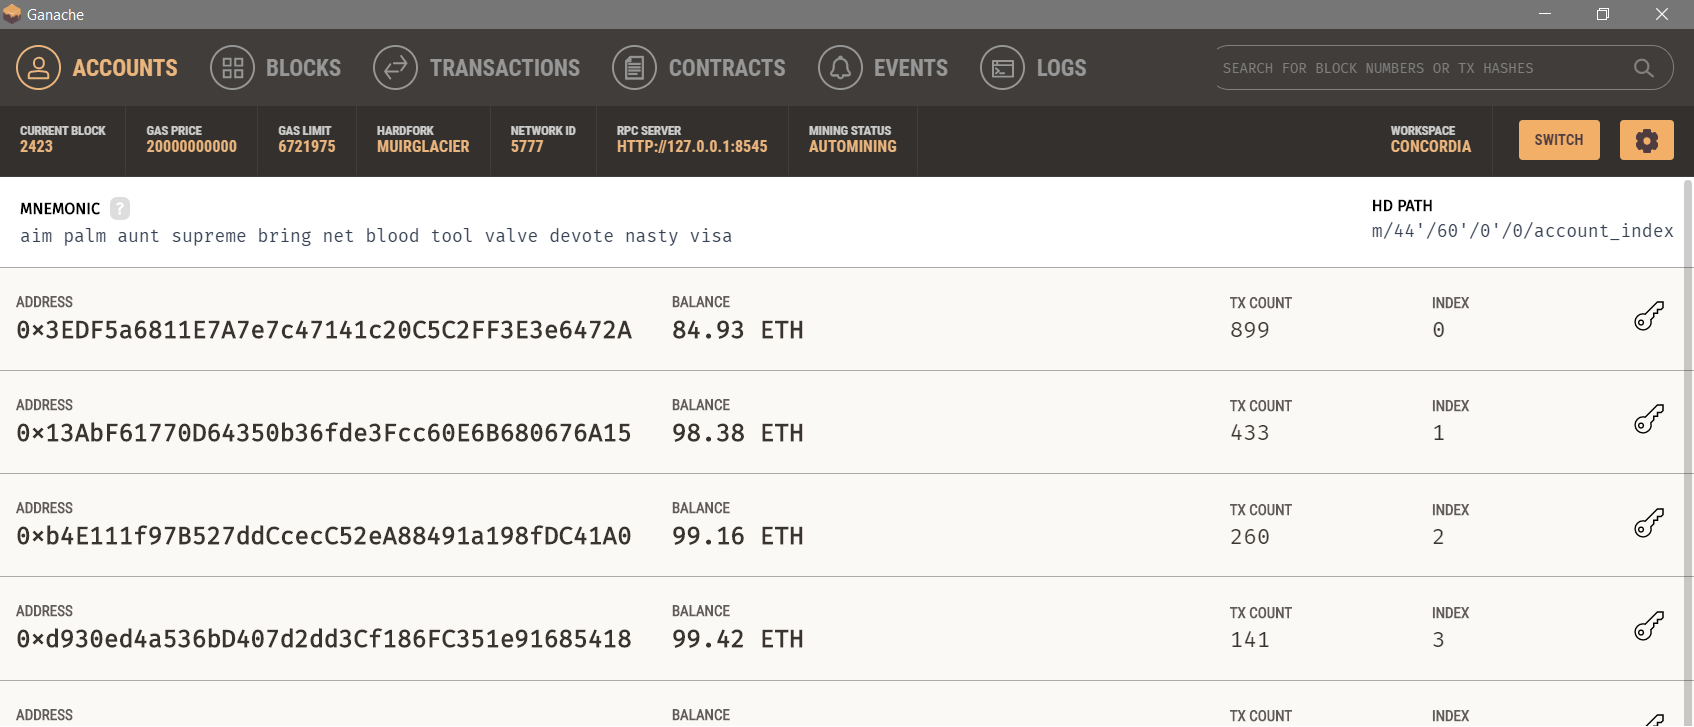
\includegraphics[width=.95\textwidth]{assets/figures/chapter-4/4.3.ganache-gui}
	\caption{Ganache (desktop εφαρμογή)}
\end{figure}

Το αποθετήριο του Ganache του βρίσκεται στο GitHub (\url{https://github.com/trufflesuite/ganache}) και διατίθεται μέσω του μητρώου npm (\url{https://www.npmjs.com/package/ganache}).
